\chapter{Experiments}
\label{ch:experiments}

This section presents our experimental setup and analyzes the VLN-CE benchmark results along the three design axes. Section~\ref{sec:exp_setup} details the training and evaluation protocols, followed by our analyses of teacher model selection (Section~\ref{sec:exp_teacher}), information flow directionality (Section~\ref{sec:exp_direction}), and temporal stride of navigation history (Section~\ref{sec:exp_stride}).

\section{Experimental Setup}
\label{sec:exp_setup}

\textbf{Training Setup.} All models were trained exclusively on the R2R and RxR training splits without external data. We performed rank-64 LoRA fine-tuning across the entire MLLM excluding the visual encoder. Key training hyperparameters are summarized in Table~\ref{tab:hyperparams}.

\begin{table}[t]
    \centering
    \caption{Training Hyperparameters}
    \label{tab:hyperparams}
    \begin{tabular}{ll}
        \toprule
        Item & Setting \\
        \midrule
        MLLM & Qwen3-VL-4B-Instruct \\
        LoRA hyperparameters & Rank 64, alpha 128, dropout 0.05 \\
        Optimizer & AdamW \\
        Peak learning rate & $2 \times 10^{-4}$ \\
        Weight decay & 0 \\
        Learning rate schedule & 2\% linear warmup followed by cosine decay \\
        Gradient clipping & 1.0 \\
        Training duration & 1 epoch, 1,481 optimizer updates \\
        GPUs & 8 NVIDIA A30 and 4 NVIDIA H100 configurations \\
        Effective batch size & 64 \\
        KD loss weight ($\lambda$) & 0.3 \\
        \bottomrule
    \end{tabular}
\end{table}

\textbf{Datasets and Evaluation.} All evaluations were conducted on R2R-CE and RxR-CE, continuous-environment VLN benchmarks built on the Habitat simulator. R2R-CE features relatively short-horizon navigation tasks, whereas RxR-CE evaluates longer trajectories accompanied by more complex instructions.

We report four primary metrics: Success Rate (SR), Success weighted by Path Length (SPL), Oracle Success Rate (OSR), and Navigation Error (NE). SR measures the fraction of episodes in which the agent stops within the target radius, while SPL accounts for both navigation success and path efficiency. OSR denotes the fraction of episodes in which the agent enters the target radius at any point along its trajectory, and NE measures the shortest distance from the final stopping position to the goal. On RxR-CE, where path fidelity is essential, we additionally report normalized Dynamic Time Warping (nDTW) to evaluate alignment between the agent's trajectory and the ground-truth path.

\section{Impact of Teacher Model}
\label{sec:exp_teacher}

\begin{table}[t]
    \centering
    \caption{VLN Performance by Teacher Models on R2R-CE Benchmark}
    \label{tab:r2r_teachers}
    \begin{tabular}{lcccc}
        \toprule
        Teacher Model & SR (\%) $\uparrow$ & SPL (\%) $\uparrow$ & OSR (\%) $\uparrow$ & NE (m) $\downarrow$ \\
        \midrule
        Baseline (No teacher) & 36.43 & 31.40 & 48.18 & 7.40 \\
        VGGT & 36.81 (+0.38) & 31.99 & 48.56 & 7.44 \\
        Pi3 & \textbf{41.49 (+5.06)} & \textbf{36.45} & \textbf{54.92} & \textbf{6.54} \\
        DA3 & 37.36 (+0.93) & 31.90 & 49.86 & 7.14 \\
        CUT3R & 37.25 (+0.82) & 31.87 & 49.32 & 7.37 \\
        \bottomrule
    \end{tabular}
\end{table}

\begin{table}[t]
    \centering
    \caption{VLN Performance by Teacher Models on RxR-CE Benchmark}
    \label{tab:rxr_teachers}
    \begin{tabular}{lccccc}
        \toprule
        Teacher Model & SR (\%) $\uparrow$ & SPL (\%) $\uparrow$ & OSR (\%) $\uparrow$ & NE (m) $\downarrow$ & nDTW (\%) $\uparrow$ \\
        \midrule
        Baseline (No teacher) & 42.93 & 34.28 & 56.12 & 7.48 & 53.36 \\
        VGGT & 43.01 & 34.39 & 55.82 & 7.52 & 53.00 (-0.36) \\
        Pi3 & \textbf{44.81} & \textbf{36.24} & \textbf{57.51} & \textbf{7.43} & \textbf{53.87 (+0.51)} \\
        DA3 & 42.41 & 33.66 & 55.63 & 7.67 & 52.30 (-1.06) \\
        CUT3R & 42.93 & 34.17 & 55.36 & 7.78 & 52.19 (-1.17) \\
        \bottomrule
    \end{tabular}
\end{table}

Tables~\ref{tab:r2r_teachers} and~\ref{tab:rxr_teachers} compare R2R-CE and RxR-CE performance across different teacher models under the same feature distillation pipeline. On R2R-CE, distilling from Pi3 yields the largest gains across every metric over the non-distilled baseline, improving SR by 5.06 percentage points and SPL by 5.05 percentage points. On RxR-CE as well, Pi3 outperforms the baseline on all metrics, raising nDTW by 0.51 percentage points. By contrast, distilling from VGGT, DA3, or CUT3R produces only marginal improvements on R2R-CE and degrades nDTW below the baseline on RxR-CE.

This disparity stems from the degree of alignment between each teacher's prediction head and the distillation target location. Because Pi3 performs dense prediction directly from the outputs of its last two backbone blocks, it is structurally well-matched to the standard distillation objective that supervises late-layer features. Conversely, VGGT, DA3, and CUT3R are trained to decode geometry through a DPT head that aggregates features across multiple intermediate layers. Consequently, 3D geometric cues may not be sufficiently concentrated in the terminal backbone layers alone, implying that conventional final-layer distillation fails to fully harness the representational capacity of DPT-head-based teachers.

\section{Impact of Information Flow Directionality}
\label{sec:exp_direction}

\begin{table}[t]
    \centering
    \small
    \setlength{\tabcolsep}{4.5pt}
    \caption{R2R-CE Performance by Information Flow Directionality}
    \label{tab:r2r_direction}
    \begin{tabular}{lllcccc}
        \toprule
        Family & Teacher & Directionality & SR (\%) $\uparrow$ & SPL (\%) $\uparrow$ & OSR (\%) $\uparrow$ & NE (m) $\downarrow$ \\
        \midrule
        VGGT & VGGT & Bidirectional & 36.81 & 31.99 & 48.56 & 7.44 \\
        VGGT & Causal VGGT & Causal, mask-only & \textbf{36.87} & \textbf{32.05} & \textbf{49.05} & \textbf{7.40} \\
        VGGT & StreamVGGT & Causal, trained & 35.51 & 30.22 & 46.82 & 7.63 \\
        CUT3R & CUT3R revisiting & Bidirectional & 36.05 & 31.36 & 49.10 & \textbf{7.37} \\
        CUT3R & CUT3R & Causal, recurrent & \textbf{37.25} & \textbf{31.87} & \textbf{49.32} & \textbf{7.37} \\
        \bottomrule
    \end{tabular}
\end{table}

\begin{table}[t]
    \centering
    \small
    \setlength{\tabcolsep}{4.5pt}
    \caption{RxR-CE Performance by Information Flow Directionality}
    \label{tab:rxr_direction}
    \begin{tabular}{lllccccc}
        \toprule
        Family & Teacher & Directionality & SR (\%) $\uparrow$ & SPL (\%) $\uparrow$ & OSR (\%) $\uparrow$ & NE (m) $\downarrow$ & nDTW (\%) $\uparrow$ \\
        \midrule
        VGGT & VGGT & Bidirectional & \textbf{43.01} & \textbf{34.39} & \textbf{55.82} & \textbf{7.52} & \textbf{53.00} \\
        VGGT & Causal VGGT & Causal, mask-only & 41.48 & 33.12 & 54.75 & 7.88 & 51.60 \\
        VGGT & StreamVGGT & Causal, trained & 42.49 & 34.15 & 55.27 & 7.79 & 52.75 \\
        CUT3R & CUT3R revisiting & Bidirectional & 41.59 & 33.48 & 54.65 & \textbf{7.74} & \textbf{52.92} \\
        CUT3R & CUT3R & Causal, recurrent & \textbf{42.93} & \textbf{34.17} & \textbf{55.36} & 7.78 & 52.19 \\
        \bottomrule
    \end{tabular}
\end{table}

Tables~\ref{tab:r2r_direction} and~\ref{tab:rxr_direction} compare VLN-CE performance across information flow directionalities within the VGGT and CUT3R families. On R2R-CE, causal VGGT and unidirectional CUT3R achieve slightly higher SR than their respective bidirectional counterparts. However, StreamVGGT---despite being trained directly with causal attention---attains only 35.51\% SR and 30.22\% SPL, underperforming both standard VGGT and causal VGGT.

On the longer-horizon RxR-CE benchmark, causal VGGT suffers a pronounced performance drop relative to VGGT, whereas StreamVGGT recovers much of this gap, reaching 42.49\% SR and 52.75\% nDTW. This confirms that causal training mitigates the distribution mismatch induced by applying an inference-time causal mask to a bidirectionally pretrained model. Even so, StreamVGGT still falls short of bidirectional VGGT across all metrics, and the CUT3R family shows mixed trends, with unidirectional CUT3R leading in SR and SPL while bidirectional CUT3R revisiting leads in nDTW.

Overall, introducing a causally trained teacher does not yield a consistent advantage over bidirectional teachers, and relative performance varies across benchmarks and metrics. These results indicate that the directional mismatch between teacher and student attention is not a dominant bottleneck in the current VLN feature distillation pipeline.

\section{Impact of Temporal Stride}
\label{sec:exp_stride}

\begin{figure}[t]
    \centering
    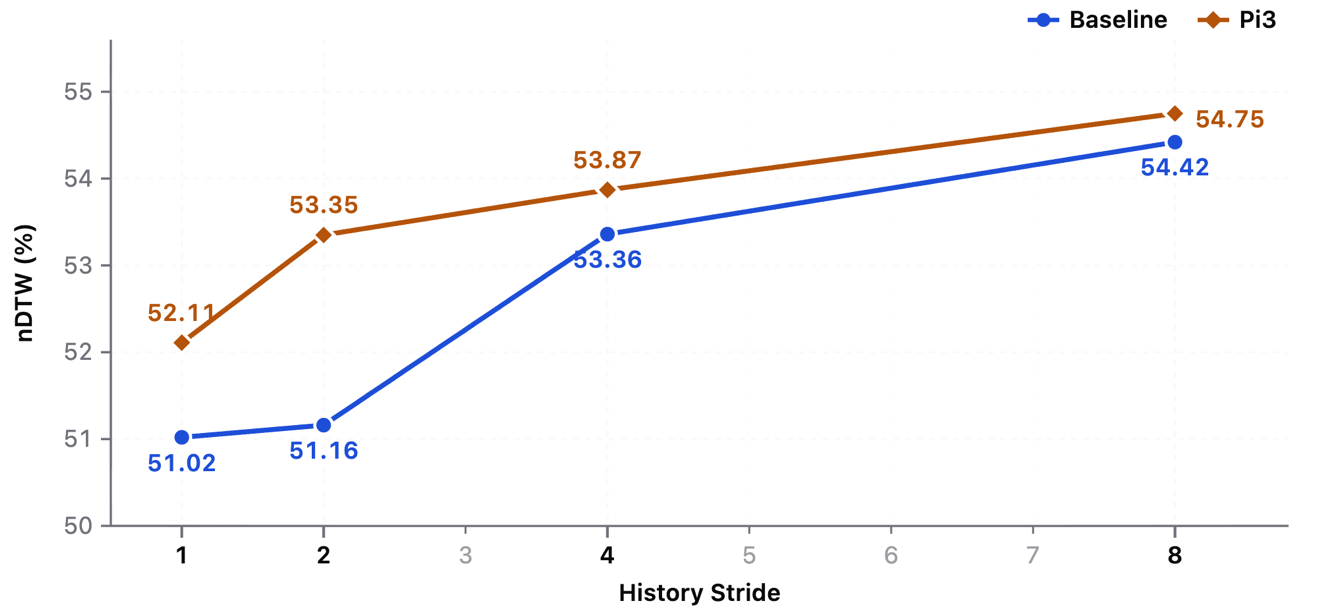
\includegraphics[width=0.85\textwidth]{figs/image1.png}
    \caption{RxR-CE nDTW (\%) across temporal strides of history}
    \label{fig:temporal_stride}
\end{figure}

We next examine how varying the temporal stride (sampling interval) affects performance while holding the number of past frames in the navigation history fixed at 8. Figure~\ref{fig:temporal_stride} plots RxR-CE nDTW for both the baseline and the Pi3-distilled model across strides of 1, 2, 4, and 8. Both models achieve steadily higher overall nDTW as the stride widens.

However, the marginal gain from distillation varies non-monotonically with stride. At stride 1, viewpoint changes between adjacent frames are minimal, providing insufficient parallax for 3D geometry inference; consequently, the gain from Pi3 distillation is smaller than at stride 2. As the stride increases from 2 to 4 and 8, the gap between the two models progressively narrows, indicating that the added benefit of geometry distillation diminishes in wide-stride regimes.

This pattern reflects a structural trade-off inherent to expanding the temporal stride. A wider stride enables a fixed frame budget to span a longer navigation history, improving the MLLM's long-horizon context comprehension. At the same time, inter-frame visual overlap drops sharply, impairing the multi-view geometry teacher's ability to establish cross-frame spatial correspondences and degrading the quality of its target features.
